% !TEX TS-program = pdflatex
% Beamer slides: Model Epidemiologi - SIR dan Variannya
% Kompilasi: pdflatex x2 (atau latexmk)
\documentclass[aspectratio=32]{beamer}

%==================== THEME ====================
\usetheme{Madrid}
\usecolortheme{seahorse}
\setbeamertemplate{navigation symbols}{} % hide nav symbols
%\setbeamertemplate{footline}[frame number]
\setbeamertemplate{footline}[author number]
\setbeamertemplate{itemize items}[circle]
\setbeamertemplate{enumerate items}[default]

%==================== PACKAGES ====================
\usepackage[T1]{fontenc}
\usepackage[utf8]{inputenc}
\usepackage{lmodern}
\usepackage{amsmath,amssymb,mathtools}
\usepackage{bm}
\usepackage{booktabs}
\usepackage{siunitx}
\usepackage{tikz}
\usetikzlibrary{arrows.meta,calc,patterns}
\usepackage{microtype}
\usepackage{xcolor}
\usepackage{hyperref}

%==================== MACROS ====================
\newcommand{\jsg}[1]{\textcolor{teal!60!black}{\textbf{#1}}}
\newcommand{\Rzero}{\mathcal R_0}
\newcommand{\dd}{\,\mathrm d}

% Nice blocks
\definecolor{myaccent}{RGB}{0,120,140}
\setbeamercolor{title}{fg=myaccent}
\setbeamercolor{frametitle}{fg=myaccent}
\setbeamercolor{block title}{bg=myaccent!10,fg=myaccent!90!black}
\setbeamercolor{block body}{bg=black!2}

% Outline at each section start
\AtBeginSection[]{
  \begin{frame}{Agenda}
    \tableofcontents[currentsection]
  \end{frame}
}

%==================== DOCUMENT ====================
\title{Model Epidemiologi: SIR dan Variannya}
\subtitle{Pemodelan Kompartemen untuk Penyakit Menular}
\title{Model Epidemiologi: SIR dan Variannya}
\author[Mohammad Jamhuri]{Dr.~Mohammad Jamhuri, M.Si}
\institute[]{Prodi Matematika FSAINTEK -- UIN Maulana Malik Ibrahim, Malang}
%\date{Pertemuan ke-4 \\ \small\today}
\date{}

\begin{document}

%-------------------- Title --------------------
\begin{frame}
  \titlepage
\end{frame}

% ================== REVIEW 1 ==================
\begin{frame}{Review: Pertumbuhan Eksponensial \& Logistik}
\small
\begin{columns}[T,totalwidth=\textwidth]
  \begin{column}{0.45\textwidth}
    \textbf{Eksponensial}\\[2pt]
    \[
      \frac{dN}{dt} = rN
      \quad\Rightarrow\quad
      N(t)=N_0 e^{rt}
    \]
    \begin{itemize}
      \item $r$: laju pertumbuhan bersih.
      \item Waktu pelipatan: $T_2=\ln 2 / r$.
      \item Cocok untuk fase awal saat sumber daya melimpah.
    \end{itemize}
  \end{column}
  \begin{column}{0.55\textwidth}
    \textbf{Logistik}\\[2pt]
    \[
      \frac{dN}{dt} = rN\!\left(1-\frac{N}{K}\right),
      \quad
      N(t)=\frac{K}{1+\left(\frac{K-N_0}{N_0}\right)e^{-rt}}
    \]
    \begin{itemize}
      \item $K$: \jsg{daya dukung} (carrying capacity).
      \item Titik belok di $N=\tfrac{K}{2}$, laju maksimum $=\tfrac{rK}{4}$.
      \item Membatasi pertumbuhan saat sumber daya terbatas.
    \end{itemize}
  \end{column}
\end{columns}
\end{frame}

% ================== REVIEW 2 ==================
\begin{frame}{Review: Lotka--Volterra (Predator--Prey)}
\small
\[
\dot{x} = a x - b x y,
\qquad
\dot{y} = -c y + d x y,
\]
\begin{itemize}
  \item $x$: prey, $y$: predator;\; $a$: pertumbuhan prey;\; $c$: kematian predator;\\
        $b,d$: intensitas interaksi.
  \item \textbf{Kesetimbangan}: $(0,0)$ dan $\big(\tfrac{c}{d},\,\tfrac{a}{b}\big)$.
  \item \textbf{Perilaku klasik}: \jsg{osilasi} populasi (fase tertinggal predator terhadap prey);\\
        di model dasar $\Rightarrow$ \textit{cycles} netral di sekitar titik koeksistensi.
  \item \textbf{Intuisi}: prey naik $\Rightarrow$ predator bertambah (karena pakan),\\
        predator tinggi $\Rightarrow$ prey turun, lalu predator turun, dan siklus berulang.
\end{itemize}
\end{frame}

%-------------------- TOC --------------------
\begin{frame}{Daftar Isi}
  \tableofcontents
\end{frame}

%=======================================================
\section{Pendahuluan}
%=======================================================

\begin{frame}{Motivasi}
Matematika \jsg{membantu memahami pola} penyebaran penyakit menular.
\begin{itemize}
  \item Wabah tidak acak belaka; ada struktur kuantitatif yang bisa dimodelkan.
  \item Tonggak: Kermack--McKendrick (1927) $\Rightarrow$ \jsg{model SIR}.
  \item Relevansi modern: COVID-19, evaluasi intervensi (vaksinasi, pembatasan kontak, karantina).
\end{itemize}
\end{frame}

\begin{frame}{Gagasan Inti}
Model kompartemen mereduksi dinamika kompleks menjadi \jsg{Sistem ODE} sederhana.
\begin{block}{Pertanyaan kunci}
\begin{itemize}
  \item Bagaimana penyakit mulai menyebar?
  \item Kapan dan pada level berapa puncak kasus terjadi?
  \item Apakah penyakit padam atau menjadi endemik?
\end{itemize}
\end{block}
\end{frame}

%=======================================================
\section{Kompartemen dalam Epidemiologi}
%=======================================================

\begin{frame}{Pembagian Kompartemen}
\begin{columns}[T,totalwidth=\textwidth]
  \begin{column}{0.55\textwidth}
    \begin{itemize}
      \item $S(t)$: \jsg{Susceptible} (rentan)
      \item $I(t)$: \jsg{Infected} (terinfeksi dan menular)
      \item $R(t)$: \jsg{Recovered/Removed} (kebal/meninggal)
    \end{itemize}
    Populasi total konstan: $N=S+I+R$.
  \end{column}
  \begin{column}{0.45\textwidth}
    \centering
    
  \end{column}
\end{columns}

\vspace{1em}

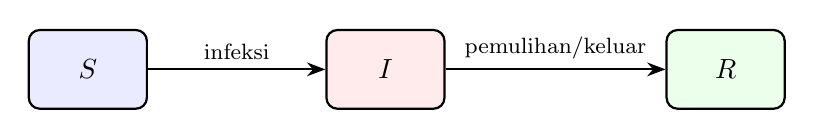
\begin{tikzpicture}[>=Stealth,thick,scale=0.9]
      \node[draw,rounded corners,minimum width=1.5cm,minimum height=1cm,fill=blue!8] (S) at (0,0) {$S$};
      \node[draw,rounded corners,minimum width=1.5cm,minimum height=1cm,fill=red!8]  (I) at (4.2,0) {$I$};
      \node[draw,rounded corners,minimum width=1.5cm,minimum height=1cm,fill=green!8] (R) at (9,0) {$R$};
      \draw[->] (S) -- node[above]{\footnotesize infeksi} (I);
      \draw[->] (I) -- node[above]{\footnotesize pemulihan/keluar} (R);
    \end{tikzpicture}
\vspace{0.5em}

\small \textit{Contoh}: kota berpenduduk 10.000; awalnya hampir semua di $S$, segelintir di $I$; seiring waktu massa berpindah dari $S\to I\to R$.
\end{frame}

%=======================================================
\section{Model SIR}
%=======================================================

\begin{frame}{Formulasi Persamaan SIR}
Asumsi interaksi proporsional: laju infeksi $\propto SI$ (laju penularan $\beta$), laju pemulihan $\gamma$.
\begin{align*}
\frac{\dd S}{\dd t} &= -\beta SI, \\
\frac{\dd I}{\dd t} &= \beta SI - \gamma I, \\
\frac{\dd R}{\dd t} &= \gamma I.
\end{align*}
\begin{block}{Makna parameter}
$\beta$: laju kontak efektif menular;\quad $\gamma$: laju pemulihan ($1/\gamma$ = lama sakit rata-rata).
\end{block}
\end{frame}

\begin{frame}{Interpretasi Biologis}
\begin{enumerate}
  \item $\dot S=-\beta SI$: $S$ turun karena tertular.
  \item $\dot I=\beta SI-\gamma I$: kompetisi infeksi baru vs pemulihan.
  \item $\dot R=\gamma I$: $R$ naik sebanding jumlah pasien aktif.
\end{enumerate}
\vspace{0.5em}
\small Contoh: $N=1000$, $I(0)=1$, $\beta=0.3$, $\gamma=0.1$. \; Awal epidemi: $\dot I(0)\approx 0.3\cdot 999-0.1\approx 299.6$ (pertumbuhan sangat cepat).
\end{frame}

\begin{frame}{Bilangan Reproduksi Dasar ($\Rzero$)}
Fase awal: $\displaystyle \dot I \approx (\beta S(0)-\gamma)I$.
\begin{equation*}
\Rzero = \frac{\beta S(0)}{\gamma}.
\end{equation*}
\begin{columns}[T,totalwidth=\textwidth]
  \begin{column}{0.58\textwidth}
    \begin{itemize}
      \item $\Rzero>1$ $\Rightarrow$ wabah tumbuh.
      \item $\Rzero<1$ $\Rightarrow$ wabah padam.
    \end{itemize}
  \end{column}
  \begin{column}{0.42\textwidth}
    \begin{block}{Ambang epidemi}
      Pertumbuhan berhenti saat $\beta S=\gamma$ $\Rightarrow$ $S=\gamma/\beta$.
    \end{block}
  \end{column}
\end{columns}
\end{frame}

\begin{frame}{Dinamika Wabah: Tiga Fase}
\begin{enumerate}
  \item \jsg{Fase awal}: $S\approx N$, $I$ naik (hampir) eksponensial.
  \item \jsg{Fase puncak}: saat $S=\gamma/\beta$, $\dot I=0$ (kasus maksimum).
  \item \jsg{Fase akhir}: $I$ turun, $R$ naik; wabah mereda, sebagian $S$ tersisa.
\end{enumerate}
\end{frame}

\begin{frame}{Sketsa Kurva $S(t), I(t), R(t)$}
\centering
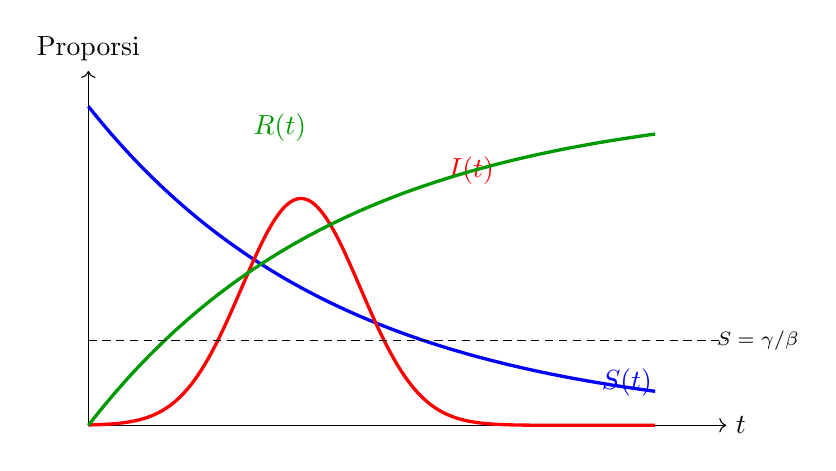
\begin{tikzpicture}[scale=0.9]
  \draw[->] (0,0) -- (9,0) node[right] {$t$};
  \draw[->] (0,0) -- (0,5) node[above] {Proporsi};
  % S(t)
  \draw[smooth,domain=0:8,samples=120,variable=\x,blue,very thick]
    plot (\x,{4.5*exp(-0.28*\x)});
  \node[blue] at (7.6,0.6) {$S(t)$};
  % I(t)
  \draw[smooth,domain=0:8,samples=120,variable=\x,red,very thick]
    plot (\x,{3.2*exp(-((\x-3)^2)/1.4)});
  \node[red] at (5.4,3.6) {$I(t)$};
  % R(t)
  \draw[smooth,domain=0:8,samples=120,variable=\x,green!60!black,very thick]
    plot (\x,{4.6*(1-exp(-0.28*\x))});
  \node[green!60!black] at (2.7,4.2) {$R(t)$};
  % threshold line S = gamma/beta
  \draw[densely dashed] (0,1.2) -- (9,1.2) node[pos=0.97,anchor=west]{\scriptsize $S=\gamma/\beta$};
\end{tikzpicture}
\end{frame}

%=======================================================
\section{Varian Model Epidemiologi}
%=======================================================

\begin{frame}{Model SIS}
Tidak ada kekebalan permanen: $S \leftrightarrow I$.
\begin{align*}
\dot S &= -\beta SI + \gamma I, \\
\dot I &= \beta SI - \gamma I.
\end{align*}
\begin{itemize}
  \item Individu pulih kembali ke $S$.
  \item Memungkinkan \jsg{endemisitas} tanpa wabah besar.
\end{itemize}
\end{frame}

\begin{frame}{Model SEIR}
Tambahkan fase \jsg{terpajan} ($E$) dengan masa inkubasi rata-rata $1/\sigma$.
\begin{align*}
\dot S &= -\beta SI, &
\dot E &= \beta SI - \sigma E, \\
\dot I &= \sigma E - \gamma I, &
\dot R &= \gamma I.
\end{align*}
\begin{itemize}
  \item Menangkap \jsg{penundaan} munculnya kasus aktif.
  \item Relevan untuk penyakit dengan inkubasi nyata.
\end{itemize}
\end{frame}

\begin{frame}{Sketsa Kurva SEIR}
\centering

\begin{figure}
    \centering
    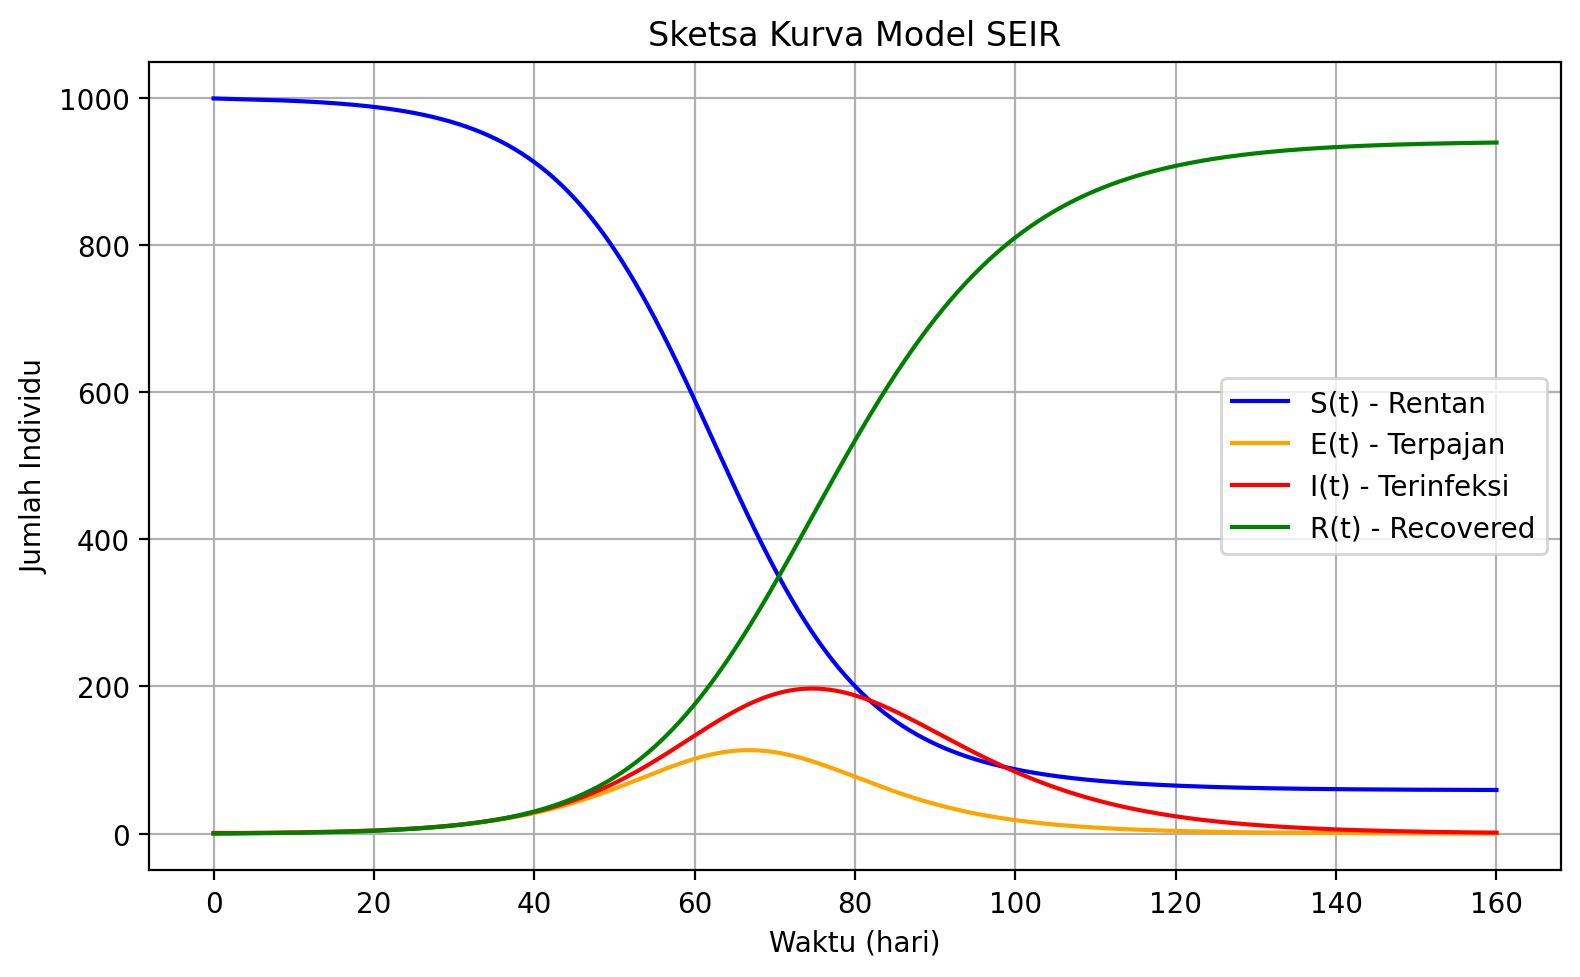
\includegraphics[width=0.75\linewidth]{image.png}
    \caption{Bentuk kurva konseptual—menunjukkan delay $E$ sebelum $I$, $S$ menurun, $R$ naik.}
    \label{fig:placeholder}
\end{figure}

\end{frame}

\begin{frame}{Model dengan Vaksinasi}
Vaksinasi laju $v$: perpindahan langsung $S\to R$.
\begin{align*}
\dot S &= -\beta SI - vS, \\
\dot R &= \gamma I + vS.
\end{align*}
\begin{block}{Imunitas Kelompok (Herd Immunity)}
Menaikkan proporsi kebal $\Rightarrow$ menurunkan $R_t$ hingga $<1$.
\end{block}
\end{frame}

%=======================================================
\section{Contoh Numerik}
%=======================================================

\begin{frame}{Parameter dan Kondisi Awal}
\begin{columns}[T,totalwidth=\textwidth]
  \begin{column}{0.55\textwidth}
  \begin{itemize}
    \item $N=1000$, $S(0)=999$, $I(0)=1$, $R(0)=0$.
    \item $\beta=0.3$, $\gamma=0.1$.
  \end{itemize}
  \end{column}
  \begin{column}{0.45\textwidth}
    \begin{block}{Bilangan Reproduksi Dasar}
      $\displaystyle \Rzero=\frac{\beta S(0)}{\gamma}=\frac{0.3\times 999}{0.1}\approx 2997$ (ilustratif).
    \end{block}
  \end{column}
\end{columns}
\small Awal: $\dot I(0) = 0.3\cdot 999 - 0.1 \approx 299.6$ $\Rightarrow$ pertumbuhan cepat.
\end{frame}

%=======================================================
\section{Keterbatasan Model Sederhana}
%=======================================================

\begin{frame}{Keterbatasan}
\begin{itemize}
  \item \jsg{Populasi homogen}: tingkat kontak dianggap sama.
  \item \jsg{Tanpa struktur spasial}: perbedaan daerah diabaikan.
  \item \jsg{Parameter konstan}: perubahan perilaku/intervensi tidak dimodelkan.
  \item \jsg{Tanpa demografi}: kelahiran/kematian alami tidak masuk.
\end{itemize}
\end{frame}

%=======================================================
\section{Model dengan Vaksinasi}
%=======================================================

\begin{frame}{SIR dengan Vaksinasi (dasar)}
\begin{itemize}
  \item Individu rentan ($S$) bisa berpindah langsung ke kebal ($R$) melalui vaksinasi.
  \item Anggap vaksinasi sempurna (efikasi 100\%), tanpa demografi.
\end{itemize}
\[
\begin{aligned}
\dot S &= -\beta \tfrac{S I}{N} \;-\; vS, \\
\dot I &= \beta \tfrac{S I}{N} \;-\; \gamma I, \\
\dot R &= \gamma I \;+\; vS.
\end{aligned}
\]
\begin{block}{Interpretasi}
$v$: laju vaksinasi. Semakin besar $v$, semakin cepat $S$ berkurang $\Rightarrow$ wabah bisa padam lebih dini.
\end{block}
\end{frame}

%-------------------------------------------------------

\begin{frame}{Model SIRV dengan Kompartemen Vaksin}
\begin{columns}[T,totalwidth=\textwidth]
  \begin{column}{0.75\textwidth}
    \begin{itemize}
      \item Tambah kompartemen $V$: tervaksin.
      \item Efikasi $\varepsilon_s$: mengurangi kerentanan.
      \item Ada peluruhan kekebalan: $\omega_V, \omega_R$.
      \item Demografi masuk lewat $\mu$ (kelahiran/kematian alami).
    \end{itemize}
  \end{column}
  \begin{column}{0.25\textwidth}
    \centering
    
  \end{column}
\end{columns}

\vspace{1em}

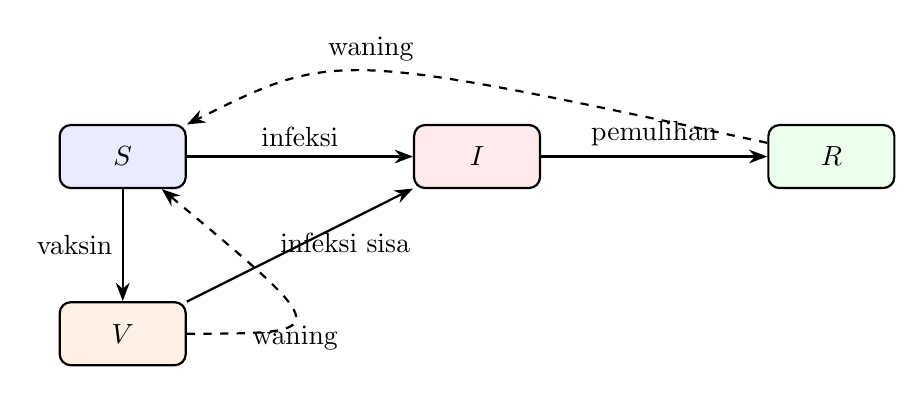
\begin{tikzpicture}[>=Stealth,thick,scale=0.9]
      \node[draw,rounded corners,fill=blue!8,minimum width=1.6cm,minimum height=0.8cm] (S) at (0,0) {$S$};
      \node[draw,rounded corners,fill=orange!10,minimum width=1.6cm,minimum height=0.8cm] (V) at (0,-2.5) {$V$};
      \node[draw,rounded corners,fill=red!8,minimum width=1.6cm,minimum height=0.8cm] (I) at (5,0) {$I$};
      \node[draw,rounded corners,fill=green!8,minimum width=1.6cm,minimum height=0.8cm] (R) at (10,0) {$R$};
      \draw[->] (S) -- node[above]{infeksi} (I);
      \draw[->] (I) -- node[above]{pemulihan} (R);
      \draw[->] (S) -- node[left]{vaksin} (V);
      \draw[->] (V) -- node[below,pos=0.7]{infeksi sisa} (I);
      \draw[->,dashed] (V) .. controls (3,-2.5) .. node[below]{waning} (S);
      \draw[->,dashed] (R) .. controls (3,1.5) .. node[above]{waning} (S);
    \end{tikzpicture}
\end{frame}

%-------------------------------------------------------

\begin{frame}{Persamaan Model SIRV}
Dengan gaya infeksi $\lambda = \beta \tfrac{I}{N}$:
\[
\begin{aligned}
\dot S &= \mu N - \lambda S - vS + \omega_R R + \omega_V V - \mu S, \\
\dot V &= vS - (1-\varepsilon_s)\lambda V - \omega_V V - \mu V, \\
\dot I &= \lambda S + (1-\varepsilon_s)\lambda V - \gamma I - \mu I, \\
\dot R &= \gamma I - \omega_R R - \mu R.
\end{aligned}
\]
\begin{block}{Catatan}
\begin{itemize}
  \item $v$: laju vaksinasi. 
  \item $\varepsilon_s$: efikasi mengurangi risiko infeksi.
  \item $\omega_R, \omega_V$: peluruhan kekebalan alami/vaksin.
\end{itemize}
\end{block}
\end{frame}

%-------------------------------------------------------

\begin{frame}{Implikasi Kebijakan}
\begin{itemize}
  \item Reproduksi efektif:
  \[
    R_t = \frac{\beta}{\gamma+\mu} \cdot \frac{S + (1-\varepsilon_s)V}{N}.
  \]
  \item Ambang cakupan vaksin (kasus vaksin sempurna):
  \[
    p_c > 1 - \frac{1}{R_0}.
  \]
  \item Strategi: percepat laju vaksinasi $v$, tingkatkan efikasi, cegah peluruhan kekebalan $\Rightarrow$ herd immunity lebih mudah dicapai.
\end{itemize}
\end{frame}

%=======================================================
\section{SEIR dengan Vaksinasi dan Karantina (SEIRVK)}
%=======================================================

\begin{frame}{Gagasan Model}
\small
Kompartemen: $S$ (rentan), $E$ (laten), $K$ (karantina laten), $I$ (infeksius komunitas), $R$ (removed), $V$ (tervaksin). \\
Parameter kunci:
\begin{itemize}
  \item $\beta$: laju kontak menular; $\gamma$: laju pemulihan; $\sigma$: laju keluar dari laten $E$.
  \item $v(t)$: laju vaksinasi ($S\!\to\!V$), efikasi terhadap infeksi $\varepsilon_s\in[0,1]$.
  \item $q(t)$: laju masuk karantina ($E\!\to\!K$), $\sigma_K$: laju keluar dari $K$.
  \item $\alpha\in[0,1]$: fraksi “bocor” dari $K$ yang kembali ke komunitas saat menjadi infeksius ($\alpha\!=\!0$ karantina sempurna).
  \item Opsional: $u(t)\in[0,1]$ (pembatasan kontak); $\mu$ demografi; $\omega_R,\omega_V$ peluruhan kekebalan.
\end{itemize}
\end{frame}

%-------------------------------------------------------

\begin{frame}{Diagram Alir}
\centering
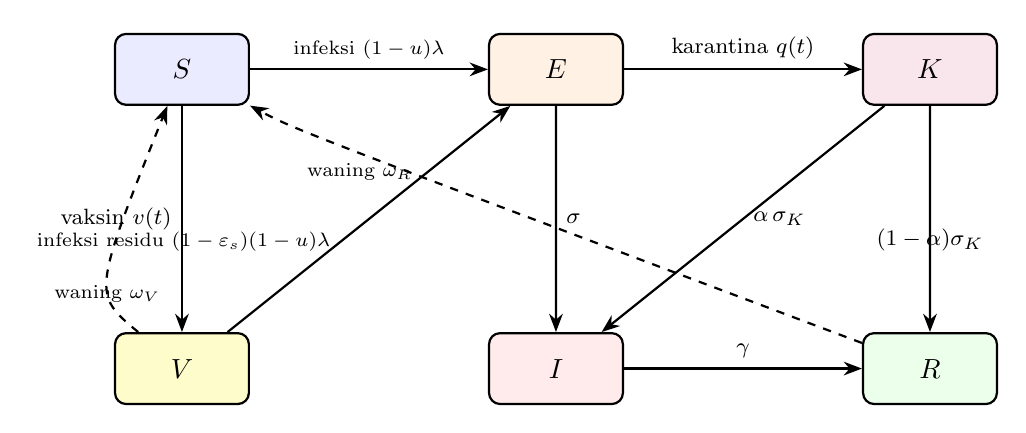
\begin{tikzpicture}[>=Stealth,thick,scale=0.95]
  \node[draw,rounded corners,fill=blue!8,minimum width=1.7cm,minimum height=0.9cm] (S) at (0,0) {$S$};
  \node[draw,rounded corners,fill=yellow!20,minimum width=1.7cm,minimum height=0.9cm] (V) at (0,-4) {$V$};
  \node[draw,rounded corners,fill=orange!10,minimum width=1.7cm,minimum height=0.9cm] (E) at (5,0) {$E$};
  \node[draw,rounded corners,fill=purple!10,minimum width=1.7cm,minimum height=0.9cm] (K) at (10,0) {$K$};
  \node[draw,rounded corners,fill=red!8,minimum width=1.7cm,minimum height=0.9cm] (I) at (5,-4) {$I$};
  \node[draw,rounded corners,fill=green!8,minimum width=1.7cm,minimum height=0.9cm] (R) at (10,-4) {$R$};

  % Infection flows
\draw[->] (S) -- (E) node[pos=0.5,above]{\scriptsize infeksi $(1-u)\lambda$};
\draw[->] (V) -- (E) node[pos=0.4,left]{\scriptsize infeksi residu $(1-\varepsilon_s)(1-u)\lambda$};

  % Vaccination
  \draw[->] (S) -- node[left]{\footnotesize vaksin $v(t)$} (V);

  % Progression & quarantine
  \draw[->] (E) -- node[right]{\footnotesize $\sigma$} (I);
  \draw[->] (E) -- node[above]{\footnotesize karantina $q(t)$} (K);

  % From quarantine
  \draw[->] (K) -- node[right]{\footnotesize $\alpha\,\sigma_K$} (I);
  \draw[->] (K) -- node[below]{\footnotesize $(1-\alpha)\sigma_K$} (R);

  % Recovery
  \draw[->] (I) -- node[above]{\footnotesize $\gamma$} (R);

  % Optional waning (dashed)
  \draw[->,dashed] (R) .. controls (1.5,-0.8) .. node[below]{\scriptsize waning $\omega_R$} (S);
  \draw[->,dashed] (V) .. controls (-1.2,-3) .. node[below]{\scriptsize waning $\omega_V$} (S);
\end{tikzpicture}

\small Gaya infeksi: $\displaystyle \lambda(t)=\beta\,\frac{I}{N}$, lalu dikalikan faktor pembatasan $(1-u(t))$ bila ada NPIs.
\end{frame}

%-------------------------------------------------------

\begin{frame}{Persamaan SEIRVK}
\small
Dengan $\lambda=\beta\,\dfrac{I}{N}$ dan (opsional) faktor $(1-u)$:
\[
\begin{aligned}
\dot S &= \mu N - (1-u)\lambda\,S - v(t)S + \omega_R R + \omega_V V - \mu S,\\[2pt]
\dot V &= v(t)S - (1-\varepsilon_s)(1-u)\lambda\,V - \omega_V V - \mu V,\\[2pt]
\dot E &= (1-u)\lambda\,S + (1-\varepsilon_s)(1-u)\lambda\,V - \sigma E - q(t)E - \mu E,\\[2pt]
\dot K &= q(t)E - \sigma_K K - \mu K,\\[2pt]
\dot I &= \sigma E + \alpha\,\sigma_K K - \gamma I - \mu I,\\[2pt]
\dot R &= \gamma I + (1-\alpha)\,\sigma_K K - \omega_R R - \mu R.
\end{aligned}
\]
\begin{itemize}
  \item $\alpha=0$: karantina sempurna (keluar $K$ langsung ke $R$, tidak ada transmisi komunitas).
  \item $\alpha>0$: kebocoran—sebagian dari $K$ kembali ke komunitas sebagai kasus infeksius.
\end{itemize}
\end{frame}

%-------------------------------------------------------

\begin{frame}{Dampak Vaksinasi \& Karantina (Heuristik $R_t$)}
\small
Secara kasar (tanpa demografi panjang \& parameter waktu-variabel):
\[
R_t \;\approx\; (1-u)\,\frac{\beta}{\gamma}\,\frac{S + (1-\varepsilon_s)V}{N}
\;\times\; \underbrace{\Bigg(\frac{\sigma}{\sigma+q}\;+\;\alpha\,\frac{q}{\sigma+q}\Bigg)}_{\text{fraksi efektif yang mencapai komunitas}}
\]
\begin{itemize}
  \item Menaikkan $q$ (karantina lebih agresif) $\Rightarrow$ kurangi fraksi yang “lolos”.
  \item Menurunkan $\alpha$ (kepatuhan karantina) $\Rightarrow$ kurangi kebocoran ke komunitas.
  \item Menaikkan $v(t)$ dan/atau $\varepsilon_s$ $\Rightarrow$ kurangi massa rentan efektif.
  \item Menaikkan $u$ (NPIs) $\Rightarrow$ kurangi kontak efektif.
\end{itemize}
\end{frame}

%=======================================================
\section{Latihan}
%=======================================================

\begin{frame}{Latihan}
\begin{enumerate}
  \item Untuk $\beta=0.2$, $\gamma=0.1$, $S(0)=500$, hitung $\Rzero$. Apakah wabah menyebar/padam?
  \item Simulasikan SIR dengan $N=1000$, $S(0)=990$, $I(0)=10$, $R(0)=0$. Gambarkan $S,I,R$ dan jelaskan.
  \item Modifikasi SEIR dengan $\sigma=1/5$ (inkubasi 5 hari). Bandingkan $I(t)$ dengan SIR.
  \item Jelaskan bagaimana vaksinasi menurunkan $\Rzero$ dan implikasi \textit{herd immunity}.
\end{enumerate}
\end{frame}

%=======================================================
\section{Penutup}
%=======================================================

\begin{frame}{Ringkasan}
\begin{itemize}
  \item SIR menangkap inti dinamika wabah: pertumbuhan awal, puncak, mereda.
  \item $\Rzero$ sebagai \jsg{ambang epidemi} dan panduan intervensi.
  \item Varian: SIS (tanpa kekebalan), SEIR (inkubasi), vaksinasi ($S\to R$).
\end{itemize}
\end{frame}


\end{document}